%version 1.00,	date 24/10/2016	auteur(s) Pierre Porche
\speaker{\Matthieu}

\begin{frame}
\frametitle{Outils techniques de qualité}
\begin{block}{Intégration dans le projet de nombreux outils d'aide au développement}
	\begin{itemize}
		\item sonarQube
		\item phpCodeSniffer %choisi par michel
		\item phpUnit (+coverage) %choisi par michel
		\item phpDocumentor
	\end{itemize}
\end{block}
\end{frame}

\begin{frame}
      \begin{figure}[r]
		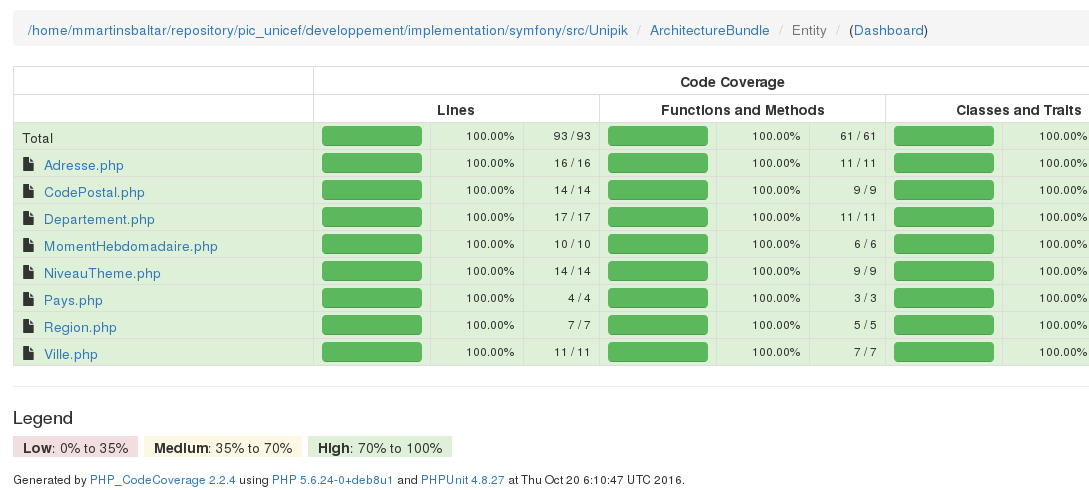
\includegraphics[scale=0.4]{images/coverage.png}
		\caption{Imprim-écran de la couverture des tests}
	  \end{figure}
\end{frame}

\begin{frame}
      \begin{figure}[r]
		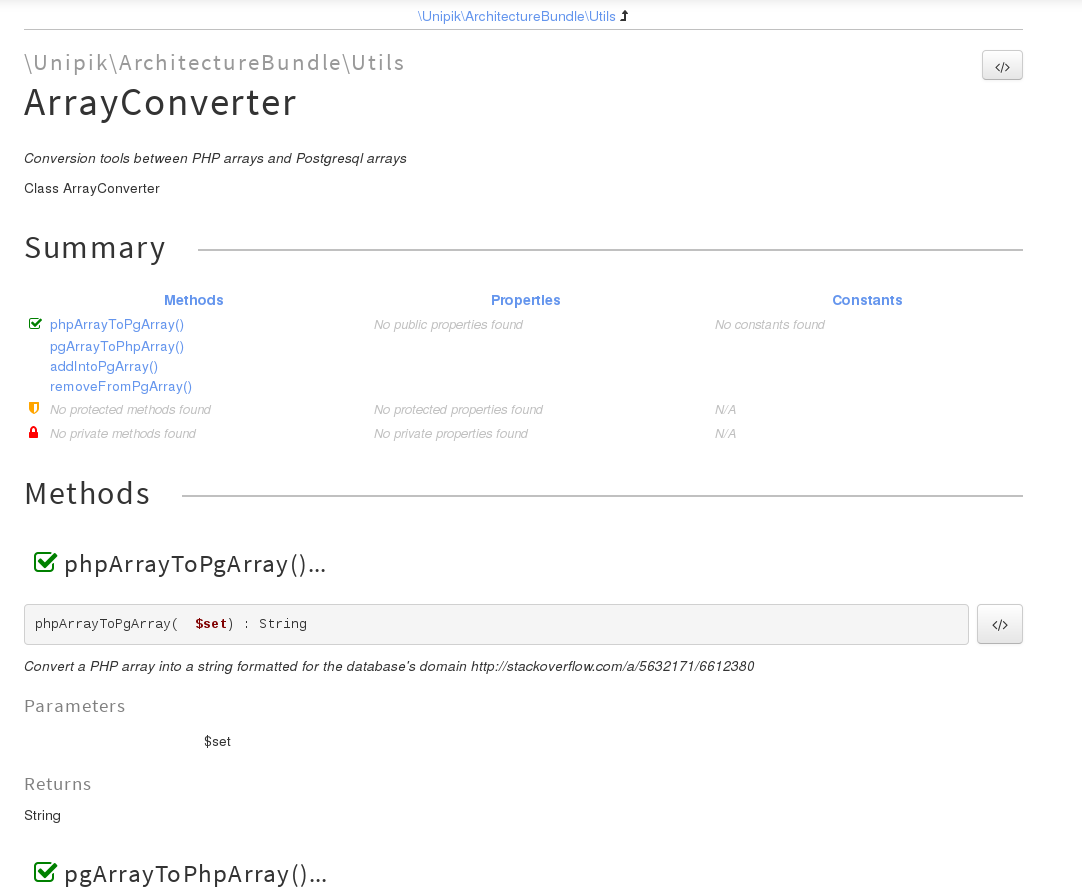
\includegraphics[scale=0.2]{images/doc.png}
		\caption{Imprim-écran de la documentation}
	  \end{figure}
\end{frame}

\begin{frame}
\frametitle{Déploiement automatiques}
\begin{block}{Environnement multiples}
	\begin{itemize}
		\item Dev: apache en local avec symlink vers le dossier de travail \\
		\emph{\tiny(http://prenom.unipik.insa-rouen.fr)}
		\item Integ: VM sur le pare-feu de la salle PIC (Vagrant) \\
		\emph{\tiny(http://integ.unipik.insa-rouen.fr)}
		\item pre-prod: machine physique dédié dans la salle pic. \\
		\emph{\tiny(http://pre-prod.unipik.insa-rouen.fr)}
		\item prod: chez digital ocean (bientôt chez quantic telecom) \\
		\emph{\tiny(http://138.68.151.59)}
	\end{itemize}
\end{block}

L'integ, la pré-prod et la prod sont approvisionnés automatiquement avec Ansible.

\end{frame}
